\documentclass[a4paper,12pt]{article}
\usepackage[slovene]{babel}
\usepackage[utf8]{inputenc}
\usepackage[T1]{fontenc}
\usepackage{lmodern}
\usepackage{amsmath}
\usepackage{hyperref} 
\usepackage{graphicx} 
\usepackage{amsfonts}
\usepackage{eurosym}
\usepackage{stackengine}
\usepackage{fancyhdr}
\usepackage{amssymb}
\usepackage{graphicx}
\usepackage{amsbsy}
\usepackage{mathtools}
\usepackage{amsthm}

\usepackage[output-decimal-marker={,}]{siunitx}

\begin{document}
\title{Robustni problem nahrbtnika}
\author{Eva Babnik in Jan Založnik}
\date{December, 2020}
\maketitle


\newpage
\tableofcontents
%\renewcommand{\listfigurename}{karkoli}
\listoffigures

\newpage
\section{Uvod}
\medskip
Namen tega poročila je, da predstaviva robustni problem nahrbtnika in kodo s katero sva ga rešila. Kodo bova sproti 
ustrezno komentirala ter dodala njeno časovno zahtevnost. Vključila bova tudi nekaj primerov in zraven dodala še časovne vrednosti, ki jih je program
potreboval za izračun rešitve. Program bova potem poskušala uporabiti na finančnem modelu. Podatke iz ameriške borze bova
uporabila na kodi za robustni problem in tako poskušala sestaviti optimalni portfelj. Prav tako bova tudi tu dodala primere in 
njihovo časovno zahtevnost.

\section{Povzetek}
\medskip
Poročilo se prične s kratko predstavitvijo navadnega oziroma klasičnega problema nahrbtnika in nato še z razlago 
robustnega problema nahrbtnika. V robustnem primer problema nahrbtnika prav tako kot pri klasičnemu problemu iščemo 
množico predmetov, ki jih bomo položili v nahrbtnik in njihovo optimalno vrednost, vendar v tem primeru nimamo točnih podatkov o 
vseh težah predmetov. Za njihove teže vemo le, da so element določenega zaprtega intervala, ki torej ima zgornjo in spodnjo mejo.
Poleg intervalov tež predmetov pa še vemo maksimalno število elementov, ki lahko spremeni svojo težo, to število označimo z $\lambda$.
\paragraph{}
Za sledeči problem sva s pomočjo dinamičnega programiranja napisala rekurzivne enačbe, na katerih bazira
najina koda v programskem jeziku \textit{python}. Napisala sva program, ki reši tako klasični problem nahrbtnika kot 
tudi robustni problem nahrbtnika in za rešitev vrne optimalni seznam predmetov, ki jih položimo v nahrbtnik in skupno 
optimalno vrednost le-teh. Sestavila pa sva tudi enostavnejši grafični program, ki omogoča, da lahko problem reši tudi posameznik, 
ki nima nikakršnega predznanja v programiranju.
\paragraph{}
Nato sva kodo malo modificirala in jo uporabila na malo poenostavljenem finančnem modelu. 
Program prebere datoteko s podatki, ki zajemajo ceno delnice, najvišjo možno ceno delnice in letno stopnjo donosa, vrne pa 
optimalni portfelj, ki si ga lahko izberemo če imamo na voljo za investicije določeno vsoto denarja.




\newpage
\section{Problem nahrbtnika}
\medskip
Klasični problem nahrbtinka (angl. \textit{classical Knapsack Problem}) je računalniški problem, s katerim poskusimo zapolniti 
nahrbtnik z danimi predmeti, ki ima vsak svojo ceno in težo. Bodisi gre za dejansko polnjenje nahrbtnika, polnjenje 
nakupovalne vreče ali morda zlaganje predmetov v avto. V nadaljevanju poročila bova za klasični problem uporabljala kar kratico KP. 
Na voljo imamo množico n-tih predmetov, ki jo označimo z $N = \{1, \dots, n\}$ in nahrbtnik s kapaciteto $c$. Vsak predmet ima 
pozitivno vrednost $p_{j}$ in pozitivno utež $w_{j}$. Problem nahrbtnika nas sprašuje, katero podmnožico predmetov iz N moramo 
položiti v nahrbtnik, da bo skupna vrednost le teh čim večja možna in da ne bo presegla nahrbtnikove kapacitete. 
Torej maksimiziramo skupno vrednost predmetov pri pogoju, da seštevek izbranih uteži ne presega nahrbtinkove zmogljivosti.
Problem lahko predstavimo kot celoštevilski linearni program (CLP):


\begin{equation}
    \tag*{}
     max \sum_{j \in N} p_{j}x_{j}
\end{equation}
\begin{equation}
    \tag*{}
    \sum_{j \in N} w_{j}x_{j} \leq c
\end{equation}
\begin{equation}
    \tag*{}
    x_{j} \in \{0,1\}, j \in N
\end{equation}

\medskip
\noindent Kjer $x_{j}$ zavzame vrednost 1, če j-ti predmet položimo v nahrbtnik,
 sicer zavzame vrednost 0. 

\section{Robustni problem nahrbtnika}
\medskip
Robustni problem nahrbtnika (angl. \textit{Robust Knapsack Problem}) v nadaljevanju 
RKP, je nekakšna nadgranja problema nahrbtnika. Dodaten problem se pojavi pri točnosti 
naših podatkov, in sicer pri utežeh $w_{j}$. Vsak predmet $j$ ima svojo nominalno težo 
$w_{j}$, ki pa je lahko netočna, ampak zanjo vemo, da se nahaja na intervalu 
[$w_{j} - \underline{w}_{j}$, $w_{j} + \overline{w}_{j}$]. Podan imamo tudi celošteviski parameter $\Gamma$,
ki označuje največje možno število predmetov z netočno izmerjeno težo. Pri iskanju 
rešitve problema moramo torej paziti, da bo seštevek vseh novih uteži še vedno manjši od
kapacitete nahrbtnika. Težav z rešitvijo seveda ne bomo imeli, če bodo vse dejanske uteži
nižje oziroma lažje od njene nominalne vrednosti, lahko pa se zgodi tudi najslabši možni 
izid, ko vse uteži zavzamejo zgornjo mejo intervala. Dopustno rešitev, kjer je
$J \subseteq N$ lahko formuliramo na naslednji način: 
\begin{equation}
    \tag*{}
    \sum_{j \in J}w_{j} + \sum_{j \in \hat{J}}\overline{w}_{j} \leq c,\quad \forall \hat{J} \subseteq J \; \text{in}\; |\hat{J}| \leq \Gamma 
\end{equation}


\section{Pristop z dinamičnim programiranjem}   %pobravano rumeno ker je č noter :/
\medskip
Naj bo $ \bar{z}(d, s, j) $ najvišji dobiček za dopustno rešitev s skupno težo $d$, kjer so upoštevani 
samo elementi iz množice $\{1, \dots,j\} \in N$ in samo $s$ izmed njih doseže zgornjo mejo $\hat{w}_j$. 
Naj bo $z(d, j)$ največji dobiček za dopustno rešitev s skupno težo $d$, kjer so upoštevani samo elementi 
iz množice $\{ 1,\dots,j \} \in N $ in naj jih le $\Gamma $ spremeni težo iz nominalne na zgornjo mejo $\hat{w}_j$. 
Torej velja $d = 0, 1, \dots, c$; $s = 0, 1, \dots, \Gamma$ in $ j = 0, 1, \dots, n$.
Ključna lastnost pravilnosti tega pristopa je predpostavka, da so predmeti razvrščeni po padajoči teži $\hat{w}_j$. 
Problem lahko zapišemo z naslednjimi rekurzivnimi zvezami: 
\begin{equation}  
    \tag*{}
    \begin{matrix}
    \bar{z}(d, s, j) = max\{ \bar{z}(d, s, j - 1), \bar{z}(d - \hat{w}_j, s- 1, j - 1) + p_j\} \\
    \text{za} \; \; d = 0,\dots, c; \; s = 1,\dots, \Gamma \:\: \text{in} \:\:j = 1,\dots, n. \\ 
    \\
    z(d, j) = max\{z(d, j - 1), z (d - w_j, j - 1) + p_j\} \\
    \text{za} \; \; d = 0,\dots, c\;\;\text{in}\;\: j = \Gamma + 1,\dots, n.
    \end{matrix}
\end{equation} 

\noindent Začetna vrednost je $\bar{z}(d, s, 0) = -\infty$ za $d = 0, \dots,c$ in s = $0, \dots, \Gamma$. 
Nato nastavimo $\bar{z}(0, 0, 0) = 0$. Oba zapisa sta med seboj povezana z enakostjo $z(d, \Gamma) = 
\bar{z}(d, \Gamma, \Gamma\}$ za vsak $d$. Optimalno vrednost robustnega problema nahrbtnika dobimo kot:
\begin{equation}
\tag*{}
z^{*} = max \begin{cases}
max\{z(d, n) |\; d = 1, \dots, c \\
max\{\bar{z}(d, s, n) |\; d = 1, \dots, c; \;s = 1, \dots, \Gamma -1\}
\end{cases}
\end{equation}
\medskip
kjer porabimo tudi celotno kapaciteto nahrbtnika $c^{*} \leq c$.
\par
Algoritem dinamičnega programiranja je sestavljen iz dveh korakov. V prvem koraku dobimo optimalno 
rešitev, ki vsebuje največ $\Gamma$ elementov s povečano težo. V drugem koraku pa nato dobljeno 
rešitev lahko razširimo z dodatnimi elementi z nespremenjeno težo. Algoritem lahko razdelimo na dva 
koraka, ker razvrstitev predmetov po padajoči teži $\bar{w}_j$ zagotavlja, da so v vsaki rešitvi 
elementi z najmanjšimi indeksi (torej tisti, ki so bili v nahrbtnik položeni prej) tisti, ki bodo 
dosegli večjo težo.

\section{Opis kode}
\medskip
V prilogi sva dodala kodo napisano v \textit{pythonu}, ki je ustrezno komentirana pri bolj zapletenih 
funkcijah, tukaj pa bova še podrobneje prikazala funkciji \textit{solve\_RKP} in \textit{rekurzija}, ki sta glavni komponenti
za izračun RKP. 
\medskip

\begin{figure}[hb!]
    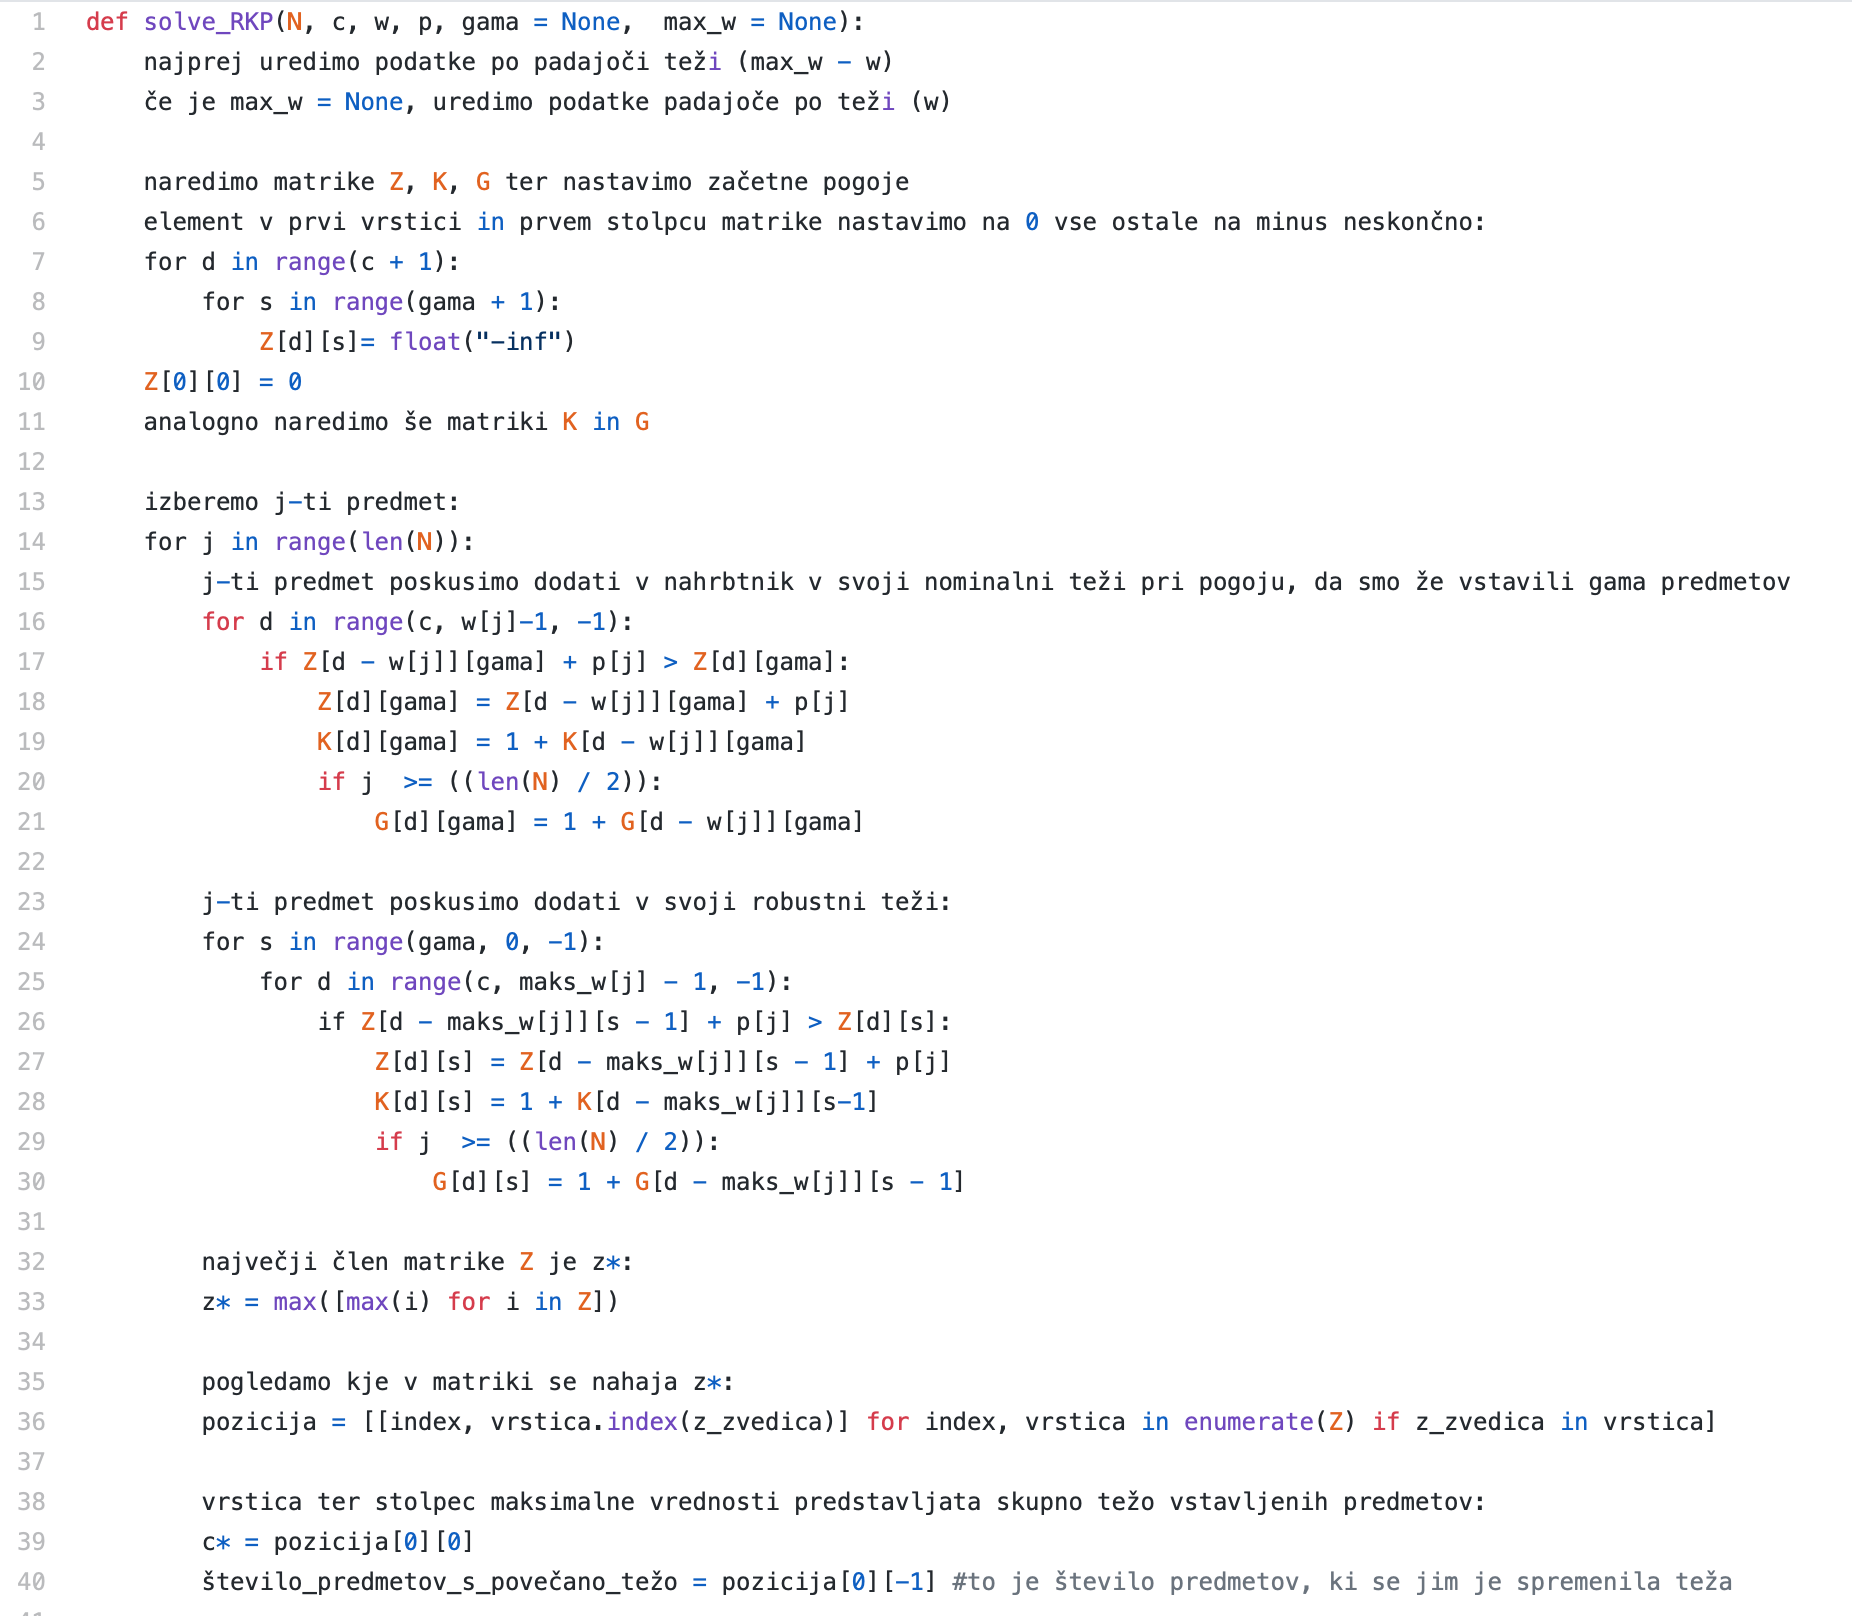
\includegraphics[width=13cm]{opis_kode1.png}
    \caption{Prvi del kode}
    \label{fig:koda1}    
\end{figure}
\paragraph{}
Funkcija \textit{solve\_RKP} sprejme štiri obvezne argumente: množico predmetov $N$ oblike
$\{1, \dots, n\}$, kjer je $n$ število predmetov; kapaciteto nahrbtnika $c$; teže predmetov $w$; vrednosti predmetov $p$ in dva neobvezna
argumenta $\Gamma$, ki označuje maksimalno število predmetov s spremenjeno težo ter $\bar{w} = max\_w$, ki prikazuje robustne teže predmetov. 
Vrne nam sledeče podatke: $z^{*}$ (optimalna vrednost predmetov, ki bodo v nahrbtniku), $c^{*}$ (optimalno težo predmetov v nahrbtniku), $k^{*}$ (število 
predmetov, ki jih damo v nahrbtnik) ter $g^{*}$ (število predmetov iz prve polovice množice $N$, ki jih dodamo v nahrbtnik). Vse te optimalne 
vrednosti potrebujemo kasneje v funkciji \textit{rekurzija}, da lahko dobimo seznam predmetov,ki jih bomo položili v nahrbtnik. V primeru ko 
ne podamo neobveznih argumentov $\Gamma$ in $max\_w$ nam funkcija \textit{solve\_RKP} vrne podobne optimalne vrednosti kot prej, le da tokrat 
reši KP.







\newpage
\section{Viri in literatura}

\begin{thebibliography}{9}

    \bibitem{RNP} 
    Michele Monaci, Ulrich Pferschy, Paolo Serafini 
    \\\texttt{https://www.sciencedirect.com/science/article/pii/S0305054813001342}


\end{thebibliography}


\end{document}
